\documentclass{beamer}
\usepackage{graphicx}
\usepackage{latexsym}
\usepackage[french]{babel}
\usepackage[utf8]{inputenc}
\usepackage[T1]{fontenc}
\usepackage{listings}
\usetheme{Frankfurt}
\title{Projet C++ : Lancer de rayons}
\author{Mathieu \textsc{Mari} \and Xavier \textsc{Montillet}}

\begin{document}

\begin{frame}
	\titlepage
\end{frame}
	
\section{Introduction}
	\begin{frame}{Introduction}
		\begin{itemize}
			\item La technique du lancer de rayons permet de générer des images 3D.
			\item Applications : Images de synthèse, jeux vidéos\dots
		\end{itemize}
	\end{frame}
\section{Principe général}
	\begin{frame}
	\begin{block}{Principe général}
	\begin{itemize}
		\item On choisit où positionner notre caméra.
		\item On choisit la position de l'écran.
		\item Pour chaque pixel d'écran, on lance un rayon partant de la caméra et passant par le pixel.
		\item On trouve le premier objet de la scene que le rayon rencontre.
		\item On calcul la couleur à renvoyer : 
			\begin{itemize}	
				\item éclairage
				\item reflexions
				\item transparence	
				\item \dots
			\end{itemize}		
	\end{itemize}
	\end{block}
	\end{frame}
	
\section{Implémentation}
	\subsection{Présentation des classes utilisées}
	\begin{frame}{Présentation des classes utilisées}
		\begin{center}
    		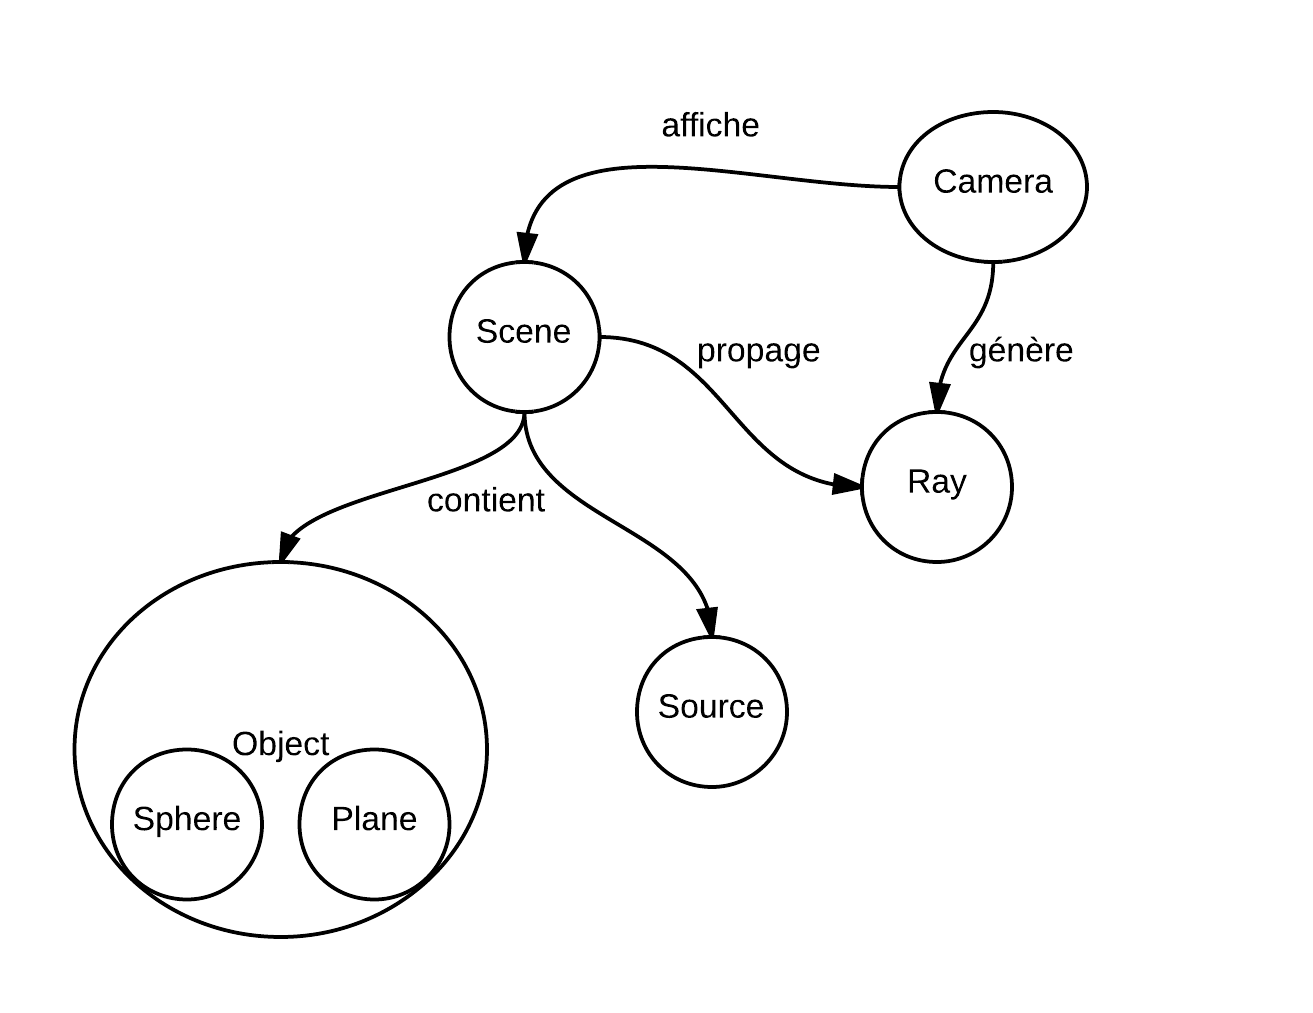
\includegraphics[height = 7cm]{schema.png}
  		\end{center}
	\end{frame}	

	\subsection{Classes auxiliaires}
	\begin{frame}
		Classes auxiliaires : 
		\begin{block}{La classe Point} 
			\begin{itemize}
				\item Contient uniquement un vecteur.
				\item Fournit une semantique plus «propre».
				\item Contrôle les relations entre points et vecteurs.
			\end{itemize}
		\end{block} \pause

		\begin{block}{La classe Option}
			\begin{itemize}
				\item Permet de detecter si il y a intersection, et de calculer en même temps la distance.
			\end{itemize}
		\end{block}
	\end{frame}
	
	\subsection{La classe Light}
	\begin{frame}{La classe Light}
		Permet de manipuler les couleurs : \emph{synthese additive\dots}
		\begin{itemize}
			\item Addition de deux couleurs composante par composante. 
			\begin{itemize}
				\item $255 \leadsto +\infty$
				\item On module par la fonction $tanh$
			\end{itemize}
			\item Addition d'une couleur et d'une lumière : une lumière.
			\begin{itemize}
				\item composante rouge $= \frac{r_{color}}{255}r_{light}$
			\end{itemize}
		\end{itemize}		
	\end{frame}

	\subsection{Comment revoyer la couleur d'un pixel ?}
		\begin{frame}{Comment renvoyer la couleur d'un pixel ?}
			\begin{itemize}
				\item Déterminer le premier objet intersécté par le rayon. 
				\item Pour chaque source éclairant le point d'intersection, multiplier la lumière de la source par la couleur de l'objet.
				\item Multiplier par le produit scalaire de la normale à l'objet et du vecteur reliant le point à la source.
				\item Additionner les lumières obtenues sur toutes les sources éclairant l'objet.
			\end{itemize}
		\end{frame}	
	
	\begin{frame}{Démonstration}
		\begin{center}		
			Démonstration !
		\end{center}
	\end{frame}

	\section{Amélioration}
		\begin{frame}{Améliorations}
			\begin{block}{Amélioration du réalisme}
				\begin{itemize}
					
					\item Réflexions, réfractions
					\item Transparence	
					\item Objets plus complexes :
					\begin{itemize}
						\item gestion de l'épaisseur.
						\item gestion de la matière.
						\item \dots
					\end{itemize}
					\item Synthèse de lois physiques plus complexes.
				\end{itemize}
			\end{block}
					
		On peut également penser à une version \og dynamique \fg du lancer de rayons.
		\end{frame}








\section{Conclusion}
	
	\begin{frame}{Conclusion}
		\begin{center}		
			Conclusion !
		\end{center}
	\end{frame}
	
\end{document}
